\chapter{Resultados}

\section{Estabilidad de estructuras}



Se estudian los posibles isómeros conformacionales de los ácidos sulfúrico, carbónico y fosfórico (ANEXO) con el fin de hallar la estructura más estable en fase gas. \\
  \begin{table}[H]
\begin{center}
\begin{tabular}{|c|c|c|c|c|c|}
\hline
Isómeros H2SO4 & \Delta E & Isómeros H2CO3 & \Delta E & Isómeros H3PO4 & \Delta E \\ \hline
H2SO4 & 4,1908 & H2CO3 & 0,0000 & H3PO4 & 0,9832 \\ \hline
H2SO41 & 2,5058 & H2CO31 & 1,3775 & H3PO41 & 0,4458 \\ \hline
H2SO42 & 0,0000 & -- & -- & H3PO42 & 0,0000 \\ \hline
-- & -- & -- & -- & H3PO43 & 0,6187 \\ \hline
\end{tabular}
\caption{Diferencias de la energía libre de Gibbs en Kcal/mol de cada isómero conformacional de los ácidos a estudiar}
\end{center}
\end{table}

A la vista de los resultados de energías expuestos en la Tabla 3.1, el isómero más estable del ácido sulfúrico es el llamado "H2SO42", debido a que dicha disposición espacial minimiza las repulsiones de los pares de electrones originando una baja energía y a su vez una mayor estabilidad, ésta también se debe a la posible formación de puentes de hidrógeno intramoleculares, ya que los hidrógenos 3 y 7 de dicho confórmero están dirigidos hacia los átomos de oxígeno 5 y 4 respectivamente, con dos pares de electrones libres en orbitales p, la distancia de los H a los O es menor que la suma de sus radios de Van Der Waals (Tabla 3.2), los H presentan una carga positiva y los oxígenos una negativa, ver Tabla 3.3.
%\begin{center}
%\begin{tabular}{c c}
%\toprule
%& Radio de Van Der Waals en \Armstrong \\
%\cmidrule{2}
%O & 1,5 \\
%\addlinespace
%H & 1,2 \\
%\bottomrule
%\end{tabular}
%\caption{Valor de los radios de Van Der Waals en \Armstrong}
%\end{center}
\begin{table}[H]
    \centering
    \begin{tabular}{|c|c|c|c|}
    \hline
         Ácido & Carga de O & Carga de H & d(O--H) \\ \hline
        H2SO4 & -0,419063 & 0,241845 & 2,78 \\ \hline
        H2SO41 & -0,456911 & 0,258090 & 2,75 \\ \hline
        H2SO42 & -0,434038 & 0,279918 & 2,49 \\ \hline
    \end{tabular}
    \caption{Parámetros para un enlace de hidrógeno}
    \label{tab:my_label}
\end{table}

El isómero del ácido carbónico más estable es el "H2CO3", los dos isómeros presentan una estructura trigonal plana, y un enlace muy fuerte CO, pero dicho confórmero posee una de las otras dos distancias CO menor que en el H2CO31, Tabla 3.4, por tanto sus enlaces son más fuertes y la molécula presenta menor energía total y mayor estabilidad, Tabla 3.1.
\begin{table}[H]
    \centering
    \begin{tabular}{|c|c|c|}
    \hline
    Ácido & d(C-OH_{(1)}) & d(C-OH_{(2)}) \\ \hline
    H2CO3 & 1,34 & 1,34  \\ \hline
    H2CO31 & 1,36 & 1,34 \\ \hline 
    \end{tabular}
    \caption{Distancias C-OH del ácido carbónico}
    \label{tab:my_label}
\end{table}

En cuanto a los isómeros del ácido fosfórico, no podemos decir que el H3PO42 sea el más estable ya que las diferencias de energía son demasiado pequeñas, y entra dentro del error que puede tener el software.

Hemos realizado el mismo estudio de estabilidad con dichos ácidos sustituyendo un y/o dos hidrógenos por un halógeno, flúor y cloro.
\begin{table}[H]
\begin{center}
\begin{tabular}{|c|c|c|c|}
\hline
Sustitución por F & \Delta E & Sustitución por Cl & \Delta E \\ \hline
HFSO4g4	& 10,818 & HClSO4g4 & 0,0555 \\ \hline
HFSO41 & 10,777 & HClSO41 & 0,0000 \\ \hline
HFSO42 & 10,780 & HClSO42 & 65,02798336 \\ \hline
HFSO43 & 10,826 & HClSO43 & 64,22690486 \\ \hline
HFSO44 & 42,675 & HClSO44 & 24,42781143 \\ \hline
HFSO45 & 10,826 & HClSO45 & 0,042670639 \\ \hline
HSO4F &	101,31 & HSO4Cl & 109,9474907 \\ \hline
SO4HF &	0,0000 & SO4HCl & 4,829939852 \\ \hline
\end{tabular}
\caption{Diferencias de la energía libre de Gibbs en Kcal/mol de cada isómero conformacional del ácido sulfurico sustituyendo un H por un halógeno}
\end{center}
\end{table}
El HClSO41 tiene dos enlace S-O muy fuerte (d(S-O)=1,43) y la disposición del cloro es tal que no hay impedimento estérico ya que está en trans con el hidrógeno.

El SO4HF es la molécula más estable en la sustitución de un hidrógeno por un flúor, ya que es la única con dos enlaces S-O muy fuertes (d(S-O)=1,43), esto es porque el flúor esta a una distancia muy grande (d(S-F)=2,52) y permite la fortaleza de los demás enlaces.

\begin{table}[H]
\begin{center}
\begin{tabular}{|c|c|c|c|}
\hline
Sustitución por F & \Delta E & Sustitución por Cl & \Delta E \\ \hline
HFCO31 & 3,9632 & HClCO3 & 48,952 \\ \hline
HFCO3 & 3,8449 & HClCO31 & 49,890 \\ \hline
HCO3F & 92,693 & HCO3Cl & 91,991 \\ \hline
CO3HF & 1,8115 & CO3HCl & 0,0000 \\ \hline
CO3HF1 & 0,0000 & CO3HCl1 & 0,3151 \\ \hline
\end{tabular}
\caption{Diferencias de la energía libre de Gibbs en Kcal/mol de cada isómero conformacional del ácido carbónico sustituyendo un H por un halógeno}
\end{center}
\end{table}

Los confórmeros más estables de este ácido sustituido con halógenos presentan distancias menores de enlaces C-O, es decir, enlaces más fuertes, por lo que poseen una energía total menor.
\begin{table}[H]
\begin{center}
\begin{tabular}{|c|c|c|c|}
\hline
Sustitución por F & \Delta E & Sustitución por Cl & \Delta E \\ \hline
H2FPO4g4 & 1,2641 & H2ClPO4g4 & 0,8643 \\ \hline
H2FPO41 & 1,2640 & H2ClPO41 & 0,8675 \\ \hline
H2FPO42 & 0,0014 & H2ClPO42 & 0,0000 \\ \hline
H2FPO44	& 8,6205 & H2ClPO43 & 40,005 \\ \hline
H2FPO43	& 8,6218 & H2ClPO44 & 40,001 \\ \hline
H2FPO45	& 56,668 & H2ClPO45 & 29,134 \\ \hline
H2FPO46	& 8,4010 & H2ClPO46 & 40,725 \\ \hline
H2FPO47	& 8,6178 & H2ClPO47 & 43,487 \\ \hline
H2FPO48	& 0,0000 & H2ClPO48 & 29,959 \\ \hline
H2FPO49	& 57,869 & H2ClPO49 & 90,161 \\ \hline
H2PO4F & 22,242 & H2PO4Cl & 1,2929 \\ \hline
PO4H2F & 23,164 & PO4H2Cl & 0,5166 \\ \hline
\end{tabular}
\caption{Diferencias de la energía libre de Gibbs en Kcal/mol de cada isómero conformacional del ácido fosfórico sustituyendo un H por un halógeno}
\end{center}
\end{table}
\section{Acidez en fase gas de moléculas}

Con el fin de estudiar el impacto de esta sustitución en la acidez en fase gas de los ácidos, se han diseñado más estructuras sustituyendo hidrógenos por fluor. Para calcular la acidez en fase gas se han hecho los mismos cálculos computacionales con sus aniones.
También se ha sustituido el grupo ácido por otro para así ver su cambio de acidez en fase gas.

 \begin{table}[H]
     \centering
     \begin{tabular}{|c|c|c|c|}
     \hline
     \multicolumn{4}{|c|}{\bfseries{ACIDEZ}} \\ \hline
     Ácido & \Delta G & \Delta G_{exp} &\Delta G_{ H. especf} \\ \hline
CF3COOH & 314,04 & 316,3 & 309,0282809\\ \hline
CF3COSH & 311,58 & 312,5 & 303,3527667\\ \hline
CF3SO3H & 292,87 & 299,5 &292,2881339\\ \hline
FHSO3 & 293,57 & 299,8 & 293,0524411\\ \hline
H2CFCOOH & 328,14 &-- & 320,5998791\\ \hline
H2CFCOSH & 323,99 & --& 314,4709262\\ \hline
H2CFSO3H & 303,60 & -- & 302,9127567\\ \hline
H2CO3 & 327,95	& -- & 319,6992767\\ \hline
H2S2O6 & 281,75 & -- & 283,4104362\\ \hline
H2SO4 & 302,60	& 302,2 & 301,2892628\\ \hline
H3CCOOH & 338,57 & -- &	328,9212264\\ \hline
H3CCOSH & 330,46 & -- &	319,4866136\\ \hline
H3CSO3H & 312,65 & 315,0 & 309,7167849\\ \hline
HCF2COOH & 	321,43 & -- & 314,9858609\\ \hline
HCF2COSH & 	316,83 & -- & 308,5712026\\ \hline
HCF2SO3H & 	297,86 & -- & 298,3781185\\ \hline
HPO3 & 303,54 & 303,3 & 300,9305154\\ \hline
HNO3 & 315,01 & 317,8 & 309,4734993\\ \hline
H3PO4 & 321,48	& -- & -- \\ \hline
     \end{tabular}
     \caption{Tabla de acideces en fase gas con y sin hidratación específica y el valor experimental en Kcal/mol.}
     \label{tab:my_label}
 \end{table}
 
 Los resultados dados en la Tabla 3.5 apoyan el siguiente orden de acidez intrínseca para los ácidos Brönsted: $ H_2S_2O_6>CF_3SO_3H>FHSO_3>HCF_2SO_3H>H_2SO_4>HPO_3>H_2CFSO_3H>CF_3COSH>H_3CSO_3H>CF_3COOH>HNO_3>HCF_2COSH>HCF_2COOH>H_3PO_4>H_2CFCOSH>H_2CO_3>H_2CFCOOH>H_3CCOSH>H_3COOH $, los ácidos llamados normalmente fuertes ($ 
 CF_{3}SO_{3}H, FHSO_{3}, HCF_{2}SO_{3}H, \\ H_{2}SO_{4}, HPO_{3}, H_{2}CFSO_{3}H $) están en un intervalo de acidez relativamente estrecho (10,7 kcal/mol), se tienen algunos valores experimentales, donde la variación con los calculados computacionalmente no llega a las 3 Kcal/mol exceptuando al $CF_3SO_3H$ y al $FHSO_3$ que difieren de 6-7 kcal/mol

La acidez aumenta cuando aumenta la tendencia del ácido a perder un protón.
Se ve como el orden de acidez sustituyendo el grupo ácido es $ COOH {<} COSH {<} SO3H $, ya que en los aniones correspondientes se debe tener en cuenta la estabilización por resonancia, deslocalización de enlaces $\pi$, que es mayor en el SO3- ya que hay mayor número de átomos, en cuanto a las otras dos estrucuras, los iones COS- y COO- son estabilización por resonancia, pero en el COS- es mayor, se puede explicar observando la carga Mulliken en dichos átomos dada en la tabla X

\begin{table}[H]
    \centering
    \begin{tabular}{|c|c|c|c|c|c|}
    \hline
    SO3^- & Carga Mulliken &COS^- & Carga Mulliken & COO^- & Carga Mulliken \\ \hline
    S & 1.007134 & S & -0.503466 & C & 0.201081 \\ \hline
    O & -0.575748 & O & -0.381057 & O & -0.482870 \\ \hline
    O & -0.575646 & C & -0.018142 & O & -0.491545 \\ \hline
    O & -0.575761 & -- & -- & -- & -- \\ \hline
    \end{tabular}
    \caption{Carga Mulliken de la moléculas CF3-grupo ácido}
    \label{tab:my_label}
\end{table}

Comparamos también sustitución de átomos de flúor por átomos de hidrógeno en el grupo CF3 de la molécula. En la Tabla 3.5 se ve que cuantos más átomos de flúor haya en la molécula mayor es su acidez, esto es por la elevada electronegatividad del flúor, cuántos más átomos de flúor haya, mayor capacidad atractora tendrá el grupo, y mayor será el efecto inductivo, polarización de carga transmitida por enlaces $\sigma$, si se observa la carga Mulliken (tabla X) en los átomos de las moléculas se comprueba su estabilización por resonancia.
\begin{table}[H]
    \centering
    \begin{tabular}{|c|c|c|c|c|c|c|c|}
    \hline
    CF_3- & Carga Mull & HCF_2- & Carga Mull & H_2CF- & Carga Mull & H_3C- & Carga Mull \\ \hline
     C & 0.549474 &  C & 0.382878 & C & 0.151906 & C & -0.189412 \\ \hline
     C & 0.201081 &  C & 0.204525 & C & 0.203532 & C & 0.234883 \\ \hline
     O & -0.482870 & O & -0.510709 & O & -0.527054 & O & -0.519973 \\ \hline
     O & -0.491545 & O & -0.488498 &  O & -0.493739 & O & -0.525498 \\ \hline
     F & -0.261497 & F & -0.287967 & F & -0.334645 &  & \\ \hline
     F & -0.261531 & F & -0.300230 &  &  &  & \\ \hline
     F & -0.253112 &  &  &  &  &  & \\ \hline
    \end{tabular}
    \caption{Carga Mulliken de moléculas grupo-COOH con las cargas de hidrógenos sumadas dentro de los átomos pesados}
    \label{tab:my_label}
\end{table}

Otro asunto muy interesante es la hidratación específica, se estudiará el impacto que tiene, en la acidez de las moléculas anteriores, la presencia de una molécula de agua en fase gas
 
A la vista de los resultados expuestos en la tabla 3.5, la acidez aumenta al haber en un punto determinado de la molécula, una molécula de agua, ya que se forman enlaces de hidrógeno fuertes como se puede comprobar mirando las distancias d(O-H) y teniendo en cuenta la existencia de un máximo de densidad en dichos enlaces.
 
\section{Obtención de propiedades termoquímicas y cálculo de acideces}

Una vez determinados los isómeros conformacionales más estables, se calculan sus acideces en fase gas mediante el cálculo de la energía libre de Gibbs de sus aniones.
La acidez en fase gaseosa de un ácido neutro y la afinidad protónica de su base aniónica se refieren a los equilibrios mostrados en la figura 3.3, los resltuados de cálculos de acidez de los ácidos se muestran en la tabla X
    \begin{figure}[h]
        \centering
        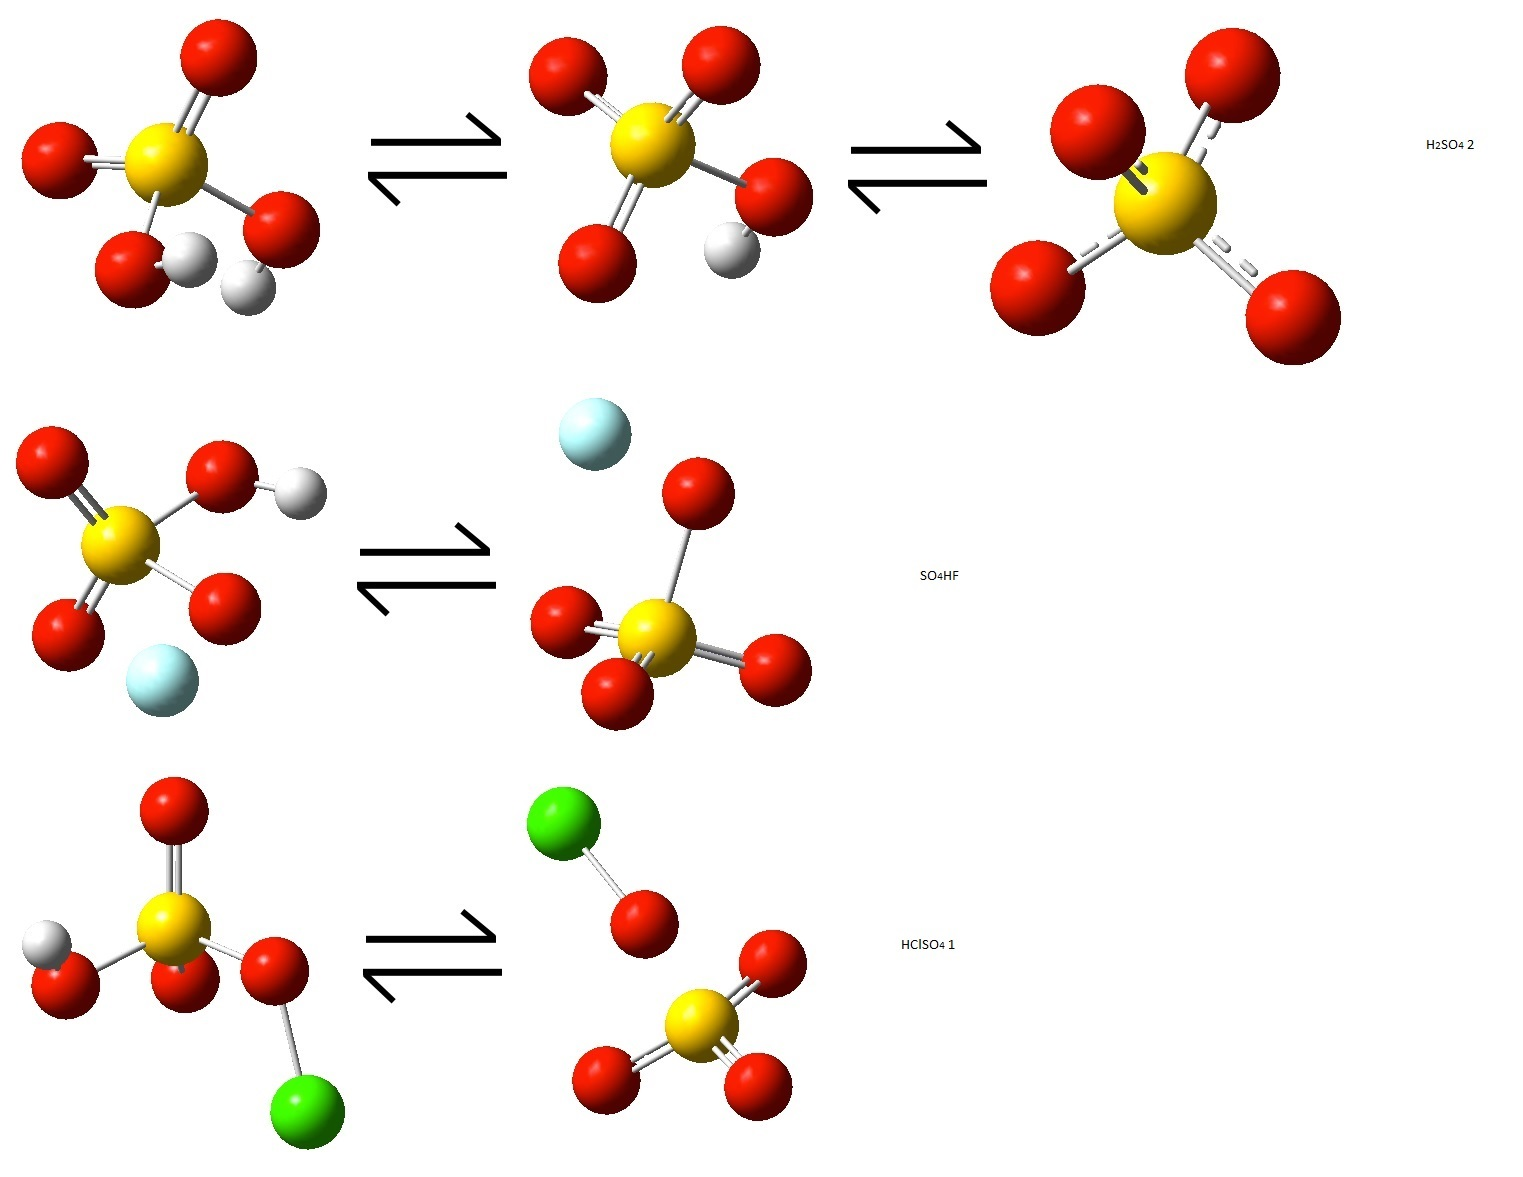
\includegraphics[scale=0.2]{EQUILIBRIOH2SO4}
        \caption{Equilibrios acido-base}
    \end{figure}

  

    
 
Las energías corregidas, entalpía y energía libre de Gibbs y la acidez en fase gas de ácidos HA se dan en la tabla X. \\
blabla \\

Los resultados de los cálculos B3LYP/6-311G** para los ácidos clásicos muestran un orden de acidez intrínseca esperado, siendo el ácido sulfúrico el más ácido
$$H_{2}CO_{3}>H_{3}PO_{4}>H_{2}SO_{4}$$ aunque el intervalo de acidez es relativamente pequeño (27.5 Kcal/mol).

Se han calculado también las energías y la acidez en fase gas de estos ácidos sustituyendo un hidrógeno por un halógeno, para así estudiar el aumento o no de su acidez al tener un elemento más electronegativo. El orden de esta acidez es $$ HFSO_{4} > HClSO_{4} > H_{2}SO_{4}$$ $$H_{2}CO_{3} > HFCO_{3} > HClCO_{3} !!!$$ $$ H_{2}ClPO_{4} > H_{3}PO_{4} > HCl_{2}PO_{4} > H_{2}FPO_{4} > HF_{2}PO_{4} $$

A partir de estos resultados se ve que dicho orden no sigue ningún patrón, por lo que la sustitución de un protón por un halógeno más o menos electronegativo no proporciona una acidez mayor, en el caso del ácido sulfúrico, al aumentar la electronegatividad del halógeno, si aumenta su acidez, pero en el caso de los otros dos ácidos no.

